\entry{2026-10-15}{Step 2: second-order stepping with the wide bank (complete)}

Lane \texttt{2026-10-13-jcp-combined}, last commit \texttt{a3c9e170d}, mirror \texttt{c51cecdbd}. Namespace \texttt{jcp-comb}, now empty; the jobs are in \texttt{runs/JOB-LEDGER.json}. There are 44 Codex audits, and the final report audit is READY. Report: \path{worktrees/2026-10-13-jcp-combined/experiments/jcp-combined/report.md}. Primary scoring is against the E0 second-order references, with E0's conditional label. First-order scores are kept beside them and stay provisional. The 3D rule selection is \textbf{post hoc} (A10, A11). Numbers are quoted from the generated report.

\subsection*{2D (38 development and validation cases)}
\begin{itemize}
\item \textbf{Selected scheme:} LSPG-CN-R. At equal cost, the accurate arm's median error falls from 0.98\,\% (BE) to 0.20\,\% (\texttt{acc} setting), and the worst from 3.0\,\% to 1.8\,\%.
\item \textbf{Bank width (H1):} R128$\to$R256 passes (median $-53.7\,\%$, 38/38 cases improve). R256$\to$R384 fails the 25\,\% bar ($-5.2\,\%$). R384$\to$R512 does not pay off.
\item \textbf{Tunability (H2):} passes.
\item \textbf{Speed against the second-order FOM (H5):} the selected scheme's best matched speed-up is 13.6$\times$. The overall best is 17.7$\times$, from an LSPG-CN arm that is not second order. The re-measured C2 \texttt{acc} arms reach 3.89$\times$. The FOM is second order in time only.
\item \textbf{H3:} the error-cancellation explanation for the fast setting's worst case is \emph{not supported}.
\item \textbf{Finalist quadrature check:} the selected arms fail it at \texttt{fast}, \texttt{acc} and R256. The fallbacks for the fast arms qualify; those for the accurate arms cost 1.3--1.6$\times$ and do not.
\end{itemize}
\begin{center}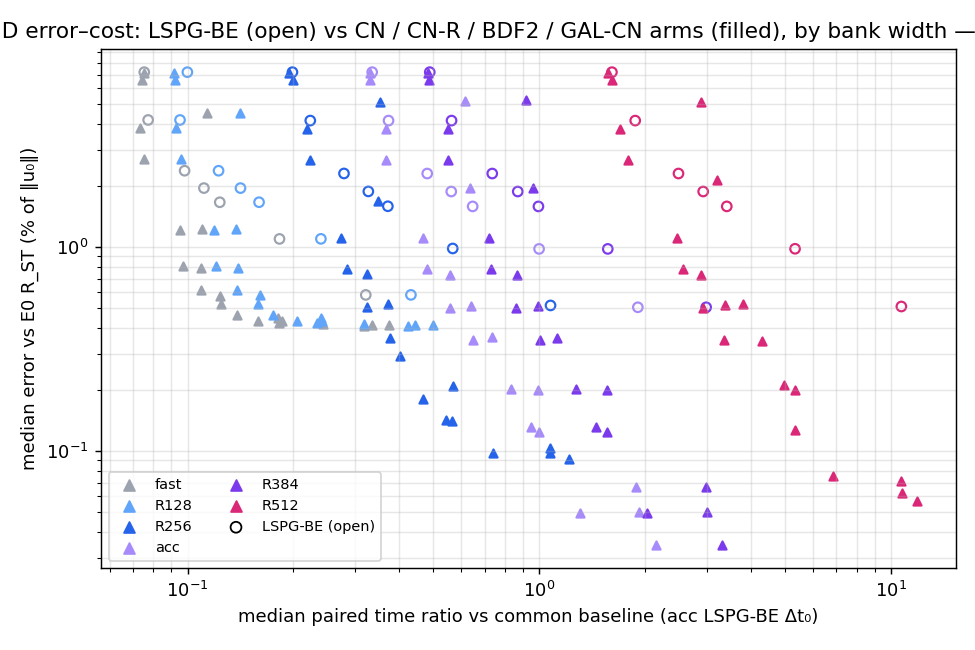
\includegraphics[width=0.48\linewidth]{figs/s2_pareto2d.png}\hfill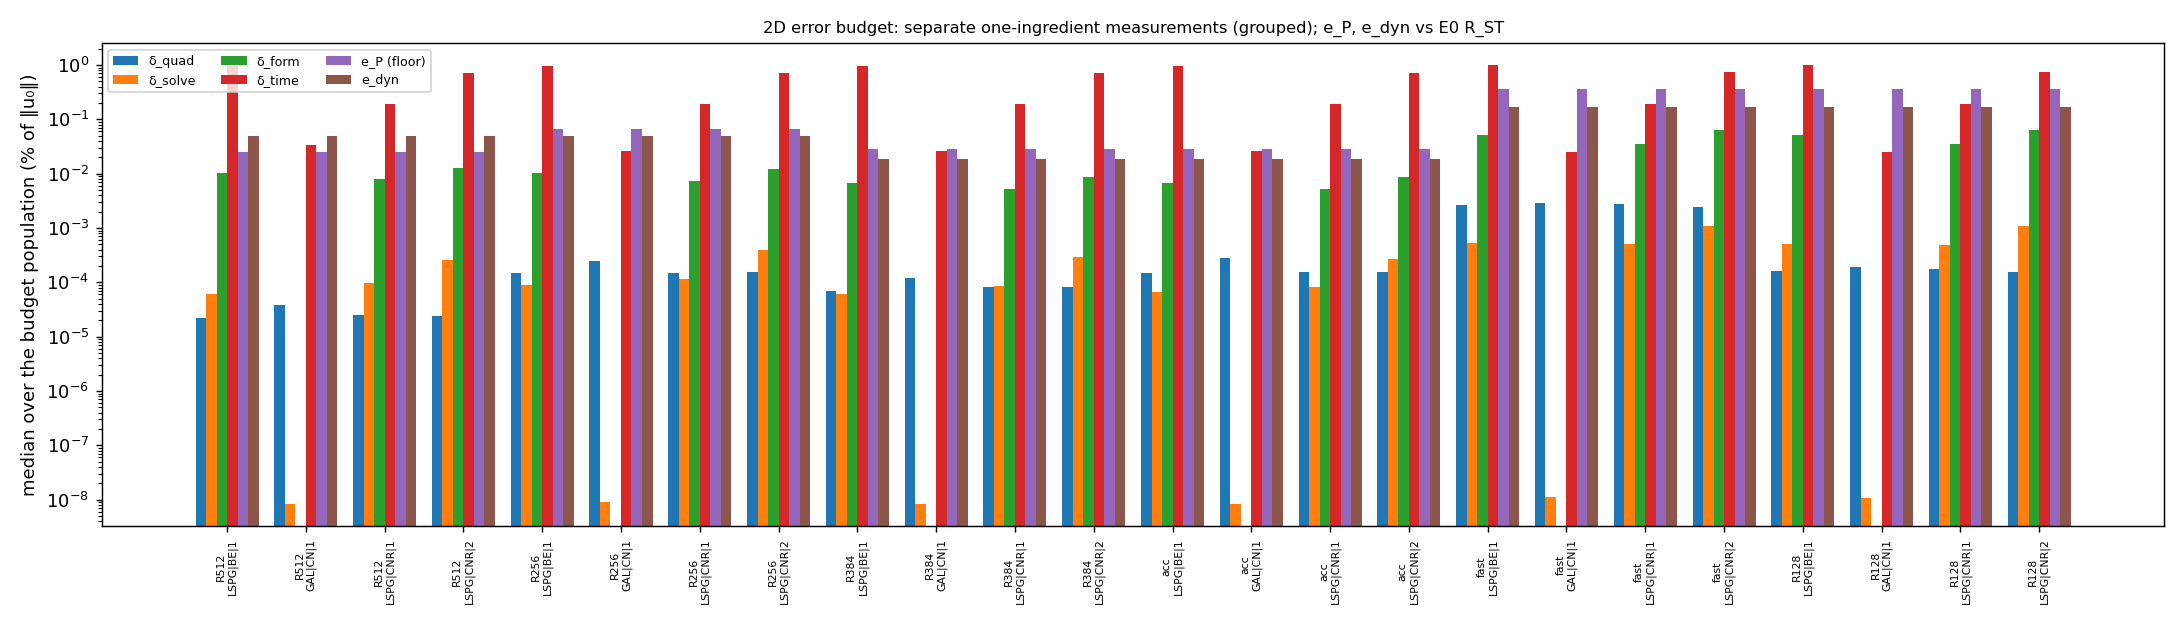
\includegraphics[width=0.48\linewidth]{figs/s2_budget2d.png}\end{center}

\subsection*{3D (validation cohort 923801, 64 cases, $65^3$)}
\begin{itemize}
\item \textbf{Accuracy at equal cost (H4b):} passes at every width. At W1024 the selected arm's median error is 0.12\,\%, against 1.53\,\% for the deployed BE. The worst errors of the selected arms are still 4.4--6.7\,\%.
\item \textbf{Speed at equal accuracy (H4a, ratio $\le 0.6$):} fails at every width. The closest equal-accuracy arms reach only 0.85--0.96.
\item \textbf{Width dial (H6):} W512$\to$W768$\to$W1024 extends (median $-60\,\%$, then $-53\,\%$). W256$\to$W512 does not.
\item \textbf{J4 gate failure at R$'\ge768$:} caused by one case (case~5). W1024 converges only at Gauss $80^3$.
\item \textbf{Fixed-sweep CN ($K{=}2$, $2.5\Delta t_0$)} fails on a fixed set of 7 cases, so the pre-registered rule selection was unavailable.
\end{itemize}
\begin{center}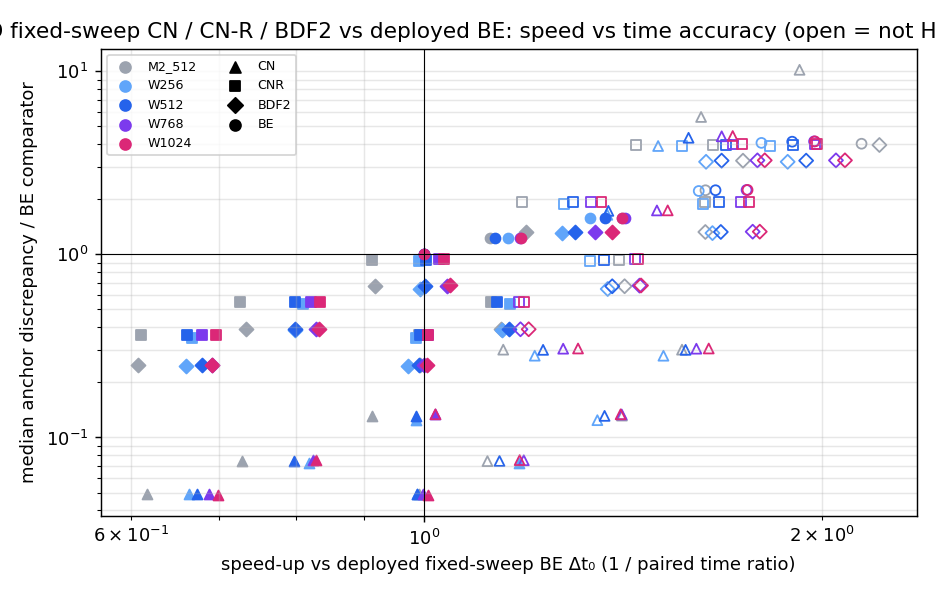
\includegraphics[width=0.6\linewidth]{figs/s2_speedup3d.png}\end{center}

\subsection*{What limits next}
Time discretisation is still the largest budget component (2D: 16 of 24 setting-arms; 3D: 13 of 19), followed by the bank's projection floor.

\subsection*{Corrections}
\retracted{The pre-registered 3D rule selection was unavailable; the one used is post hoc (A10, A11). A first frozen 3D fast-equal-accuracy selection was retracted before any budget job (A15). Some first-order H1 and H6 verdicts change under E0 (A13). Earlier drafts used second-order wording for the reduced arms and stacked non-additive budget bars. Offline scoring on the local GB10 GPU corrupted R$'$=1024 decodes, so all offline analysis now runs on CPU.}

\subsection*{Follow-up}
The 3D speed lane (\texttt{2026-10-14-jcp-speed3d}) is running. It tries one-pass Jacobian reuse at large steps, narrower banks, overhead cuts and batching, and large-mesh FOM comparisons, including a pseudo-spectral FOM.
